 \begin{figure*}[thb!]
 	\caption{Approach overview}
 	\centering
 	\label{fig:approach_overview}
 	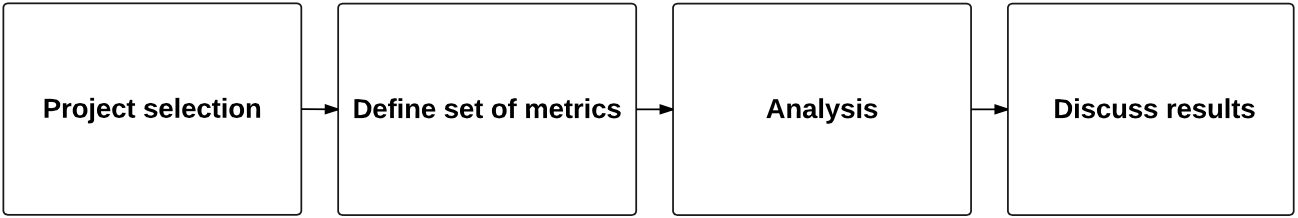
\includegraphics[width=1\textwidth]{figures/approach_overview}
 \end{figure*}
After selecting projects we have to find an automatic way to have all versions downloaded, and ready for analysis. Instead of downloading each version separately, we devise a viable and more efficient technique. We cloned latest release containing \textit{\.git} folder in it. Then we write a script to checkout each tag based on the tags that git gives us by running \textit{git tag}.
\par
Each version of each application has been analyzed with a powerful source code analyzer tool named SonarQube to extract metrics relevant to evolution of software. We also used this tool catch anti-patterns developers do in JavaScript and categorize them based on their severity.
To have all these data get analyzed in SonarQube we had to deal few unexpected behavior. For example SonarQube does not consider release dates as the real release date. It just take out the date of the analysis that it fires to analyze a source. In this scenario we have 1065 releases with the release date of the day we ran analysis. So we fixed the issue to have proper release dates.

\par After analyzing every tag in SonarQube we extract our chosen metrics that we found them proper for studying evolution of JavaScript projects. Metrics such as McCabe cyclomatic complexity,  comment line density, duplicated lines and blocks, number of directories and statements and etc. Table  \ref{tab:metrics_definition} defines sets of metrics that we used in our analysis.


\begin{table*}[!hbt]
	\begin{center}
		\caption{Release details from each analyzed project}
		\label{tab:metrics_definition}
		\begin{tabular}{c| l l }
			\toprule
			\textbf{Metric} & \textbf{Definition} \\ \midrule
			Lines of Code & The number of uncommented lines of code    \\
			Complexity      & McCabe complexity    \\
			Complexity/function & Average complexity by function. \\
			Complexity/file & Average complexity by file \\
			Comment lines  & Number of lines containing either comment or commented-out code. \\
			Comment Lines (\%)   & Density of comment lines = Comment lines / (Lines of code + Comment lines) * 100    \\
			Duplicated lines (\%)     & Density of duplication = Duplicated lines / Lines * 100    \\
			Duplicated blocks   & Number of duplicated blocks of lines    \\
			Directories   & Number of directories    \\
			Functions            & Number of functions    \\
			Statements      & Number of functions   \\
			Issues    & Number of issues with severity of blocker, critical, major and minor   \\
		SQALE Rating   & ?????????    \\
			Technical debt    & Number of days it takes to fix issues with respect to their severity    \\
			Technical debt ratio   & Division of SQALE Index by the estimation effort to re-develop your application from scratch.    \\
		\end{tabular}
	\end{center}
\end{table*}



\subsection{Project Selection}

In selecting projects for our study, we used several criteria. First, we selected projects that are popular between developers and with a large number of users, since we want to analyze their evolution, it is important that they are active projects. Second, we used projects that have their source code and issuer tracker both hosted in GitHub. This makes easier to collect information about collaboration and measure popularity of the projects. Besides, GitHub provides us an API to extract data from their repositories that will collaborate with the evolution analysis that we will run. Third we consider at this point projects with similar sizes. We will enhance this criteria with size and application domain in our final report so we can be more assertive when searching for insights about the evolution of the projects. However it is not possible to have the real-world projects with the same size in these two different languages. So we will apply some normalization approach, to make sure we are able to compare these two different worlds.

Regarding the lifespan of the analyzed projects we considered 5 previous full releases, regardless of the time that it took to be released. We consider a full release accordingly to the analyzed project. These releases are the ones with major changes in design and addition of new features as well, because of that we considered them as good candidates to conduct our study.  

As mentioned, before we ran our analysis in 10 open source projects, five of them were written in JavaScript and namely they are as following: NPM a package manager for JavaScript, Node MySQL a pure node.js JavaScript Client implementing the MySql protocol, Esprima a high performance and standard-compliant JavaScript parser, Grunt a JavaScript task runner and Node Redis a Redis client for node. Table \ref{tab:java_script_proj_details} presents hight level data of these projects.

In the same way the five Java projects analyzed were ElasticSearch is aa distributed, RESTful search engine, Gauva is the Google Core Libraries for Java 6+, JodaTime is widely used as replacement for the Java date and time classes, Jsoup is a Jason library for Java and finally JUnit is an unit test framework for Java. Their data are presented in Table \ref{tab:java_proj_details}     

\begin{table*}[!tbh]
	\begin{center}
		\caption{JavaScript Project Details }
		\label{tab:java_script_proj_details}
		\begin{tabular}{l| c c c c c}
			\toprule
			\textbf{Project} & \textbf{\# of JS files in latest release} & \textbf{Number of Directories} & \textbf{LOC\footnote{Lines of code}} & \textbf{Number of Functions} & \textbf{Number of Statements} \\ 
			\midrule
			NPM              & 165                                       & 32                             & 9,075                                & 1,217                        & 5,329                         \\
			Node MySQL       & 140                                       & 11                             & 4,720                                & 667                          & 3,317                         \\
			Esprima          & 34                                        & 6                              & 83,385                               & 4,862                        & 29,002                        \\
			Grunt            & 31                                        & 9                              & 2,361                                & 251                          & 1,245                         \\
			Node Redis       & 18                                        & 6                              & 2,529                                & 457                          & 2,537                         \\ 
			\bottomrule
		\end{tabular}
	\end{center}
\end{table*}

\begin{table*}[!tbh]
	\begin{center}
		\caption{Java Project Details }
		\label{tab:java_proj_details}
		\begin{tabular}{l| c c c c c c}
			\toprule
			\textbf{Project} & \textbf{\# of JS files in latest release} & \textbf{Number of Directories} & \textbf{LOC} & \textbf{Number of Functions} & \textbf{Classes} & \textbf{Number of Statements} \\ 
			\midrule
			ElasticSearch    & 4,050                                     & 831                            & 424,007                              & 35,762                       & 5,967            & 198,944                       \\
			Gauva            & 799                                       & 28                             & 90,401                               & 11,769                       & 1,644            & 32,698                        \\
			JodaTime         & 327                                       & 15                             & 84,855                               & 9,560                        & 473              & 50,609                        \\
			Jsoup            & 80                                        & 14                             & 13,672                               & 1,487                        & 154              & 7,980                         \\
			JUnit            & 392                                       & 73                             & 26,079                               & 3,479                        & 1,063            & 7,972                         \\ 
			\bottomrule
		\end{tabular}
	\end{center}
\end{table*}

%\begin{table*}\label{eval_table}\centering
%	\caption{Proposed experiment projects with preliminary results of most recent version of release in our dataset}
%	\begin{threeparttable}
%		\scalebox{0.7}{
%			\begin{tabular}{llccccc}
%				\toprule
%				Project & Description &  {\# of JS files in latest release} & Number of Directories & LOC \footnote{Lines of code}& Number of Functions & Number of Statements  \\
%				\addlinespace
%				\midrule
%				NPM & Package manager for JavaScript & 165 & 32 & 9,075 & 1,217 & 5,329  \\
%				\addlinespace
%				\midrule
%				Node MySQL & A pure node.js JavaScript Client implementing the MySql protocol.  & 140 & 11& 4,720 & 667 & 3,317 \\			
%				\addlinespace 	
%				\midrule
%				Esprima & A high performance, standard-compliant JavaScript parser written in JavaScript  & 34 & 6 & 83,385 & 4,862 & 29,002  \\
%				\addlinespace		
%				\midrule
%				Grunt & The JavaScript Task Runner & 31 & 9 & 2,361 & 251 & 1,245 \\
%				\addlinespace
%				\midrule
%				Node Redis & Redis client for node & 18 & 6 & 2,529 &  457 & 2,537   \\	
%				\addlinespace 
%				
%			\end{tabular}
%		}
%	\end{threeparttable}
%\end{table*}
%
%\begin{table*}\label{tab:eval_java}\centering
%	\caption{Proposed experiment projects with preliminary results of most recent version of release in our dataset}
%	\begin{threeparttable}
%		\scalebox{0.7}{
%			\begin{tabular}{llccccccc}
%				\toprule
%				Project & Description & {\# of java files in latest release} & Number of Directories & LOC & Number of Functions & classes & Number of Statements \\
%				\addlinespace
%				\midrule
%				ElasticSearch & Open Source, Distributed, RESTful Search Engine 
%				& 4,050 & 831 & 424,007 & 35,762 & 5,967 & 198,944 \\
%				\addlinespace
%				\midrule
%				Gauva & Google Core Libraries for Java 6+ & 799 & 28 & 90,401 & 11,769 & 1,644 & 32,698\\    
%				\addlinespace 
%				\midrule
%				JodaTime & Joda-Time is the widely used replacement for the Java date and time classes. & 327 & 15 & 84,855 & 9,560 & 473 & 50,609 \\
%				\addlinespace    
%				\midrule
%				Jsoup & Jason library for java & 80 & 14 & 13,672 & 1,487 & 154 & 7,980 \\
%				\addlinespace
%				\midrule
%				JUnit & Unit test framework for java & 392 & 73 & 26,079 & 3,479 & 1,063 & 7,972  \\   	
%				\addlinespace 
%			\end{tabular}
%		}
%	\end{threeparttable}
%\end{table*}

\subsection{Define set of metrics}

Lehman suggests using the number of “modules” as the best way to measure the size of a large software system \cite{Lehman1997METRICS}. However, we decided to use the number of uncommented lines of code (“uncommented LOC”) like the way Godfrey et al \cite{Godfrey2000ICMS} did the evolution study on Linux Kernel. On the other hand we measure the comment lines and the ratio of comments to lines of codes, and based on that we can infer how much developers tend to put comments within their codes. We have to consider hidden corners that can mislead results, for example descriptive comments are totally different to the lines of codes that got commented because of refactoring or changes which consider as light-weight code smells within the code.

We want to measure various aspects of the growth of these applications by having metrics such as number of files, lines of code, number of functions and statements. We also measure amount of duplications known as clones in terms of lines of codes, blocks and files. We would measure the cyclomatic complexity over time which the metric is calculated as following. Whenever the control flow of a function splits, the complexity counter gets incremented by one. Each function has a minimum complexity of 1. The control flow can split by conditional statements like if/else, switch case and so on. This metric is also known as also known as McCabe metric
We use the term “source file” to mean any file whose name ends with “.js” and also we removed folders containing external libraries which is usually located at \textit{lib} or \textit{node\_modules}. 

We also measure the amount of object oriented principles that JavaScript developers use in their day to day software development. We think if we quantify the amount of reusable parts (i.e classes) in these projects, there are some valuable reasons laid down related to evolution behind these techniques. Consequently we use a project, known as JSDeodorant to find class declarations and places developers instantiate objects.
In the rest of this section we describe how developers create objects in JavaScript and how they mimic object oriented class definitions without having direct language support in the specification of language.

\noindent\textbf{Creation Types:} Here, we explain different types of object creation no matter if they are built-in type or user-defined. 
%\subsubsection{Creation Types}

\medskip
\noindent\subsubsection{Array Literal Expression}
%\duptype{\textbf{Type I}: \textit{Array Literal Expression}.}

it creates a string array consisting of three creations possible in JavaScript elements and is assigned to variable “cars” using a binary operator (with two operand and equal operator). 
\medskip
\begin{lstlisting}[caption={Array literal expression},label={lst:array_literal},language=JavaScript]
var cars = ['Saab', 'Volvo', 'BMW'];
\end{lstlisting}
A JavaScript array is initialized with the given elements, except in the case where a single argument is passed to the Array constructor and that argument is a number. Note that this special case only applies to JavaScript arrays created with the Array constructor, not array literals created with the bracket syntax.
\\
%\break
%\duptype{\textbf{Type II}: \textit{Array Creation using \textbf{new} keyword}.}
\noindent\subsubsection{Array Creation using \textbf{new} keyword}

The Array constructor function with using the “New” keyword creates an array of three elements and then assigned the created object to variable “planes” using binary operator. Using the more verbose method: \textit{new Array()} instead of array literal expression does have one extra option in the parameters: if you pass a number to the constructor, you will get an array of that length. 

\medskip
\begin{lstlisting}[caption={Array constructor},label={lst:array_constructor},language=JavaScript]
var planes= new Array('Boeing', 'Airbus', 'Bombar- dier');
\end{lstlisting}

\noindent\subsubsection{Object Literal Expression}

%\duptype{\textbf{Type III}: \textit{Object Literal Expression}.}

The created object is basically singletons with variables/methods that are all public. An object literal is a comma-separated list of name-value pairs wrapped in curly braces. Object literals encapsulate data, enclosing it in a tidy package. This minimizes the use of global variables which can cause problems when combining code. If any of the syntax rules are broken, such as a missing comma or colon or curly brace, a JavaScript error will be triggered. No need to invoke constructors directly or maintain the correct order of arguments passed to functions.
\begin{lstlisting}[caption={Object literal expression},label={lst:object_literal_expression},language=JavaScript] 
var myObj = {
	myMethod: function(params) {
		// ...do something
	}
};
\end{lstlisting}

\noindent\subsubsection{Function Constructor}
%\duptype{\textbf{Type IV}: \textit{Function Constructor}.}

Listing \ref{lst:function_constructor}, shows the function constructor, there we define a function that should start with an uppercase letter by convention (to inform call sites use this function with “new” keyword). The Function constructor creates a new Function object and in JavaScript every function is actually a Function object.

Parameters are Names to be used by the function as formal parameter names. Each must be a string that corresponds to a valid JavaScript identifier or a list of such strings separated with a comma. Functions created with the Function constructor do not create closures to their creation contexts; they always are created in the global scope.

When running them, they will only be able to access their own local variables and global ones, not the ones from the scope in which the Function constructor was called.

\begin{lstlisting}[caption={Function constructor},label={lst:function_constructor},language=JavaScript] 
function Employee(name){
	this.name = name;
	this.getName = function(){
		return this.name;
	};	
};
var emp = new Employee ('John');
\end{lstlisting}